The extraction module encapsulates all the necessary functionality in order to extract the given user's sent messages. As it is shown in Figure \ref{fig:umlext}, this UML package has five different UML classes: \textit{Extractor}, \textit{MessageExtractor}, \textit{ThreadExtractor}, \textit{DataExtractor} and \textit{ExtractedMessage}.

\begin{figure}[p]
	\centering%
	\centerline{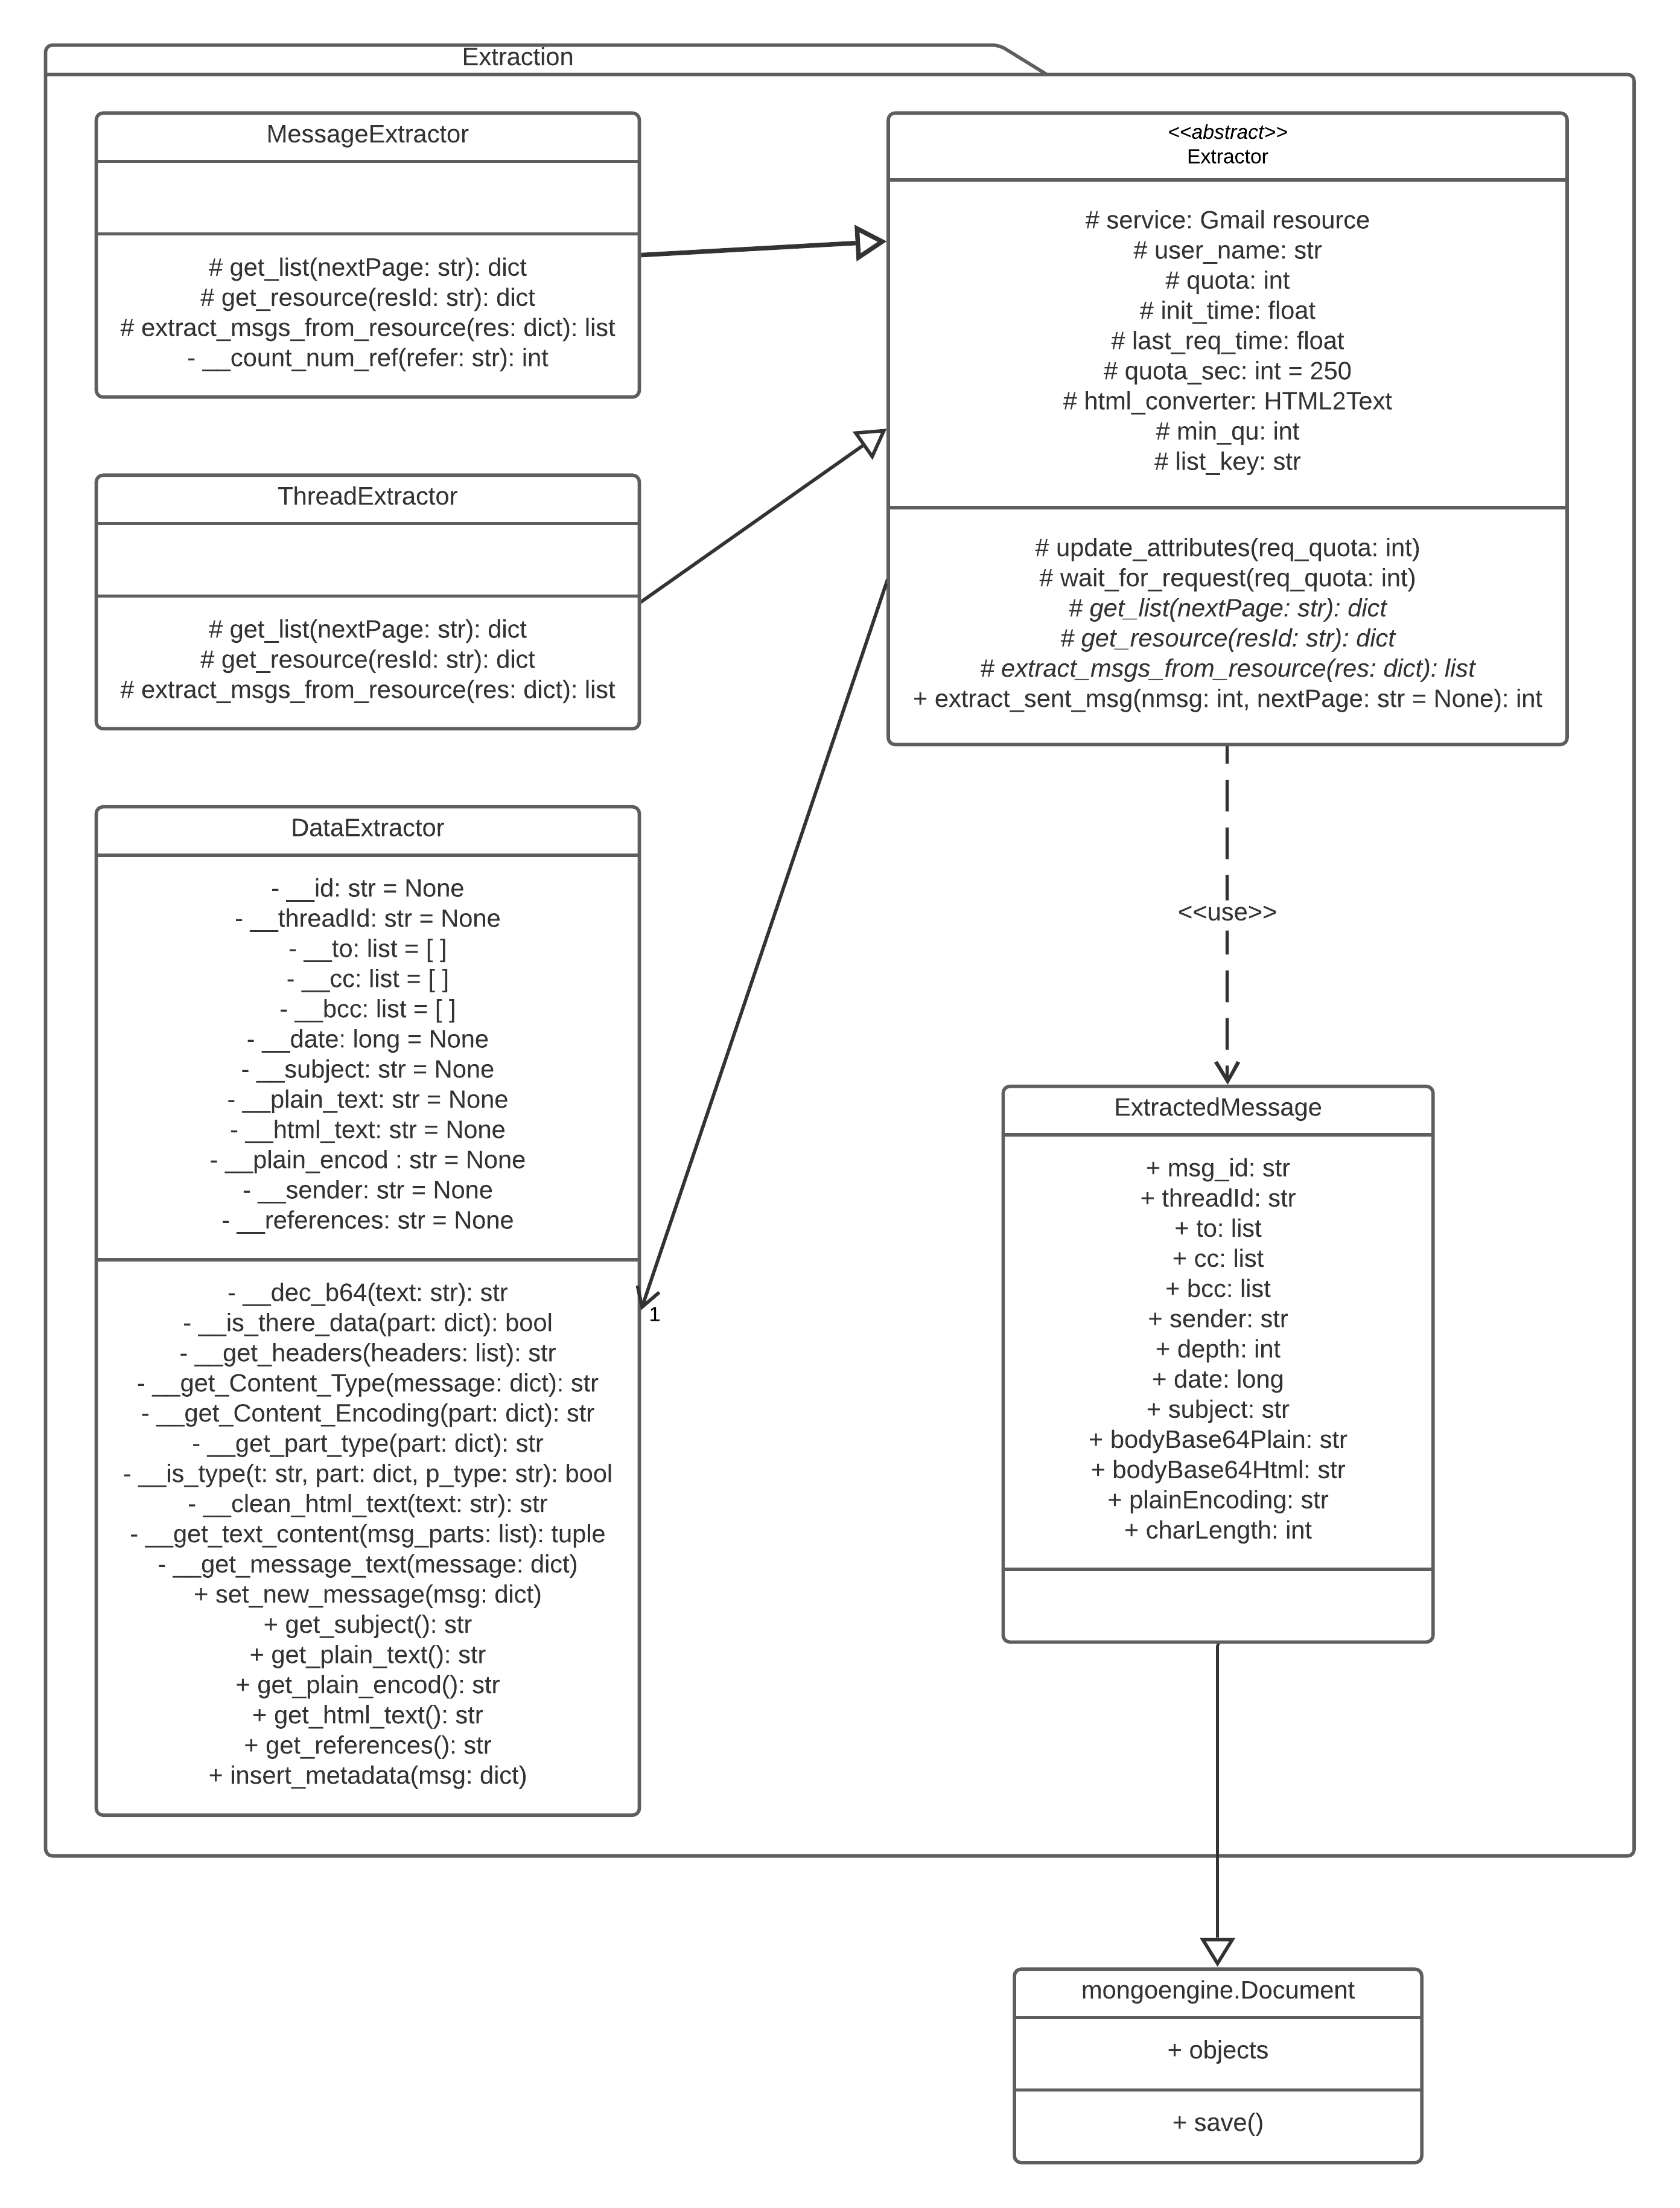
\includegraphics[width=\textwidth]{Imagenes/Bitmap/Analyser/extractionUML.png}}%
	\caption{UML class diagram of the extraction module}%
	\label{fig:umlext}
\end{figure}


The main class of the above five is the \textit{Extractor} class, which is an abstract class implemented by \textit{MessageExtractor} and \textit{ThreadExtractor} classes. The reason for implementing it as an abstract class with the abstract methods \textit{get\_list}, \textit{get\_resource} and \textit{extract\_sent\_msg}, lies in the desire to minimise the number of quota units used during this process. Let's explain this in detail.

As we have see in the Table \ref{tab:quotaUnits}, to carry out the messages resource's operation costs five quota units and to perform the same operations for the thread's resource costs ten quota units. However, when the operation \textit{messages.get} is invoked we get a single message, whereas when the operation \textit{threads.get} is called we get as many messages as there are in the thread. Therefore, minimising the amount of quota units used depends on the number of messages and threads we have.

When we are in the extraction process, at first it is necessary to invoke a \textit{list} method. It returns a list of, at least, 100 identifiers of the resource (message or thread). Then, these identifiers are used to obtain (by calling the corresponding \textit{get} method) each of the listed resources. If we want to obtain the identifiers of the remaining resources, we will have to invoke \textit{list} again with the \textit{nextTokenPage} obtained in the previous call. With this in mind, we are going to invoke the corresponding \textit{list} method as many times as the result of applying the ceiling function to the division of the number of resources by 100; and we are going to invoke the corresponding \textit{get} method as many times as the amount of resources the user has (this number is possible to know by calling the \textit{get} method of the labels resource and giving it the string value \textit{SENT} as its parameter called \textit{id}, which only consumes one quota units each time). Hence, the number of quota units inverted in an extraction process will be determined by the following formula:

$$
Q = L\cdot\left\lceil\frac{N}{100}\right\rceil+G\cdot N
$$

Where $L$ is the cost in quota units of invoking the corresponding \textit{list} method once, $N$ is the number of resources that the user has and $G$ is the cost in quota units of calling the corresponding \textit{get} method once. It is important to remember that the division is the integer and not the real one.

Following the previous expression and the quota units cost of Table \ref{tab:quotaUnits}, we are able to claim that the number of quota units inverted in a message extraction process will be:

$$
Q_M = 5\cdot\left\lceil\frac{N_M}{100}\right\rceil+5\cdot N_M
$$

Where $N_M$ is the amount of sent messages that the user has. However, the cost in quota units of a thread extraction process will be determined by:

$$
Q_T = 10\cdot\left\lceil\frac{N_T}{100}\right\rceil+10\cdot N_T
$$

Where $N_T$ is the number of sent threads that the user has. Consequently, when we obtain that $Q_M < Q_T$, we save more quota units by executing a message extraction process and, when $Q_T < Q_M$, it happens by executing a thread extraction process.

Returning to the extraction module, even though the choice between the two types of extraction is done by the Analyser (see Section \ref{sect:analyserclass}), it is necessary to implement both possibilities. For this reason, \textit{Extractor} class was implemented as an abstract class with the methods related to the \textit{list} and \textit{get} functions of the Gmail API: \textit{get\_list} (which calls the corresponding \textit{list} method) and \textit{get\_resource} (which invokes the corresponding \textit{get} method). In addition to them, we can find the \textit{extract\_msgs\_from\_resource} as an abstract method. This function is in charge of extracting the necessary information from the corresponding resource in order to obtain a list of messages (in the case of the message resource the list has only one item) which are going to be stored in the database. In other words, it transforms a message (or a thread of messages) with the structure explained in Section \ref{sssect:msgres} into the following structure (in the case of the thread resource each message is transformed to the following structure):

\begin{python}
{
	'id' : string,
	'threadId' : string,
	'to' : [ string ],
	'cc' : [ string ],
	'bcc' : [ string ],
	'sender' : string,
	'depth' : int,               # How many messages precede it
	'date' : long,               # Epoch ms
	'subject' : string,
	# Body as plain text encoded using base64
	'bodyBase64Plain' : string,
	# Body as html text encoded using base64
	'bodyBase64Html' : string,
	# Original encoding of the body as a plain text
	'plainEncoding' : string,    
	'charLength' : int
}
\end{python}

In order to carry out this structural transformation, it is necessary to go through the MIME type tree structure (see Section \ref{sssect:MIMEheaders}) and look for the different parts of the original message.

Once the message has that structure, it is ready to be saved in the database, because of, as we can observe in Figure \ref{fig:umlext}, the dictionary keys are the same as the attributes of the \textit{ExtractedMessage} class (which inherits from the \textit{mongoengine.Document} class, allowing it to insert elements in the database). Indeed, the \textit{extract\_msgs\_from\_resource} method returns a list of \textit{ExtractedMessage} objects.

In addition to the explained abstract methods, in the \textit{Extractor} class we can find the \textit{extract\_sent\_msg}, which is in charge of the extraction algorithm that we mentioned before (invoke the corresponding \textit{list} method, for each identifier get the resource, call the function \textit{extract\_msgs\_from\_resource}, etc.). During this process, the \textit{Extractor} must check that it does not exceed the set limit of quota units, both the daily limit and the secondly limit. Once the daily limit is reached, the process must stop. In the case of the secondly limit, the \textit{Extractor} must stop and wait until it can continue using the Gmail API operations. This is the task of \textit{update\_attributes} (which updates the time and quota attributes such as \textit{quota}, \textit{quota\_sec}, \textit{last\_req\_time} and \textit{init\_time}) and \textit{wait\_for\_request} methods.

In respect of the \textit{Extractor} class, there is an only remaining detail that should be mentioned. It has an attribute called \textit{html\_converter}. This attribute is an object of the \textit{HTML2Text} class from \textit{html2text} Python's library\footnote{\url{https://pypi.org/project/html2text/}}. As we need the e-mail in plain text, in case the extracted message does not have it in this format, we can use this attribute to transform the HTML text into plain text.

If we observe the \textit{Extraction} package, we will also find the \textit{DataExtractor} class, which is related with the \textit{Extractor} class by an uni-directional binary association with a multiplicity index in the arrowhead (the \textit{DataExtractor}'s end). It performs the task of extracting the information of a given e-mail. To this end, it goes through the headers list (where information as the recipient can be found) and the MIME message parts tree studied in Section \ref{sssect:MIMEheaders}, in order to get the message body. Likewise, once an e-mail is extracted from Gmail API, the \textit{DataExtractor} class receives it and acquires all the required information from it.